\hypertarget{ux4f7fux7528-list-ux548c-tuple}{%
\subsection{使用 list 和 tuple}\label{ux4f7fux7528-list-ux548c-tuple}}

\hypertarget{list}{%
\subsubsection{list}\label{list}}

Python 内置的一种数据类型是列表:list。list
是一种有序的集合,可以随时添加和删除其中的元素。

比如,列出班里所有同学的名字,就可以用一个 list 表示:

\begin{pythoncode}
>>> classmates = ['Michael', 'Bob', 'Tracy']
>>> classmates
['Michael', 'Bob', 'Tracy']
\end{pythoncode}

变量\texttt{classmates}就是一个 list。用\texttt{len()}函数可以获得 list
元素的个数:

\begin{pythoncode}
>>> len(classmates)
3
\end{pythoncode}

用索引来访问 list 中每一个位置的元素,记得索引是从\texttt{0}开始的:

\begin{pythoncode}
>>> classmates[0]
'Michael'
>>> classmates[1]
'Bob'
>>> classmates[2]
'Tracy'
>>> classmates[3]
Traceback (most recent call last):
  File "<stdin>", line 1, in <module>
IndexError: list index out of range
\end{pythoncode}

当索引超出了范围时,Python
会报一个\texttt{IndexError}错误,所以,要确保索引不要越界,记得最后一个元素的索引是\texttt{len(classmates)\ -\ 1}。

如果要取最后一个元素,除了计算索引位置外,还可以用\texttt{-1}做索引,直接获取最后一个元素:

\begin{pythoncode}
>>> classmates[-1]
'Tracy'
\end{pythoncode}

以此类推,可以获取倒数第 2 个、倒数第 3 个:

\begin{pythoncode}
>>> classmates[-2]
'Bob'
>>> classmates[-3]
'Michael'
>>> classmates[-4]
Traceback (most recent call last):
  File "<stdin>", line 1, in <module>
IndexError: list index out of range
\end{pythoncode}

当然,倒数第 4 个就越界了。

list 是一个可变的有序表,所以,可以往 list 中追加元素到末尾:

\begin{pythoncode}
>>> classmates.append('Adam')
>>> classmates
['Michael', 'Bob', 'Tracy', 'Adam']
\end{pythoncode}

也可以把元素插入到指定的位置,比如索引号为\texttt{1}的位置:

\begin{pythoncode}
>>> classmates.insert(1, 'Jack')
>>> classmates
['Michael', 'Jack', 'Bob', 'Tracy', 'Adam']
\end{pythoncode}

要删除 list 末尾的元素,用\texttt{pop()}方法:

\begin{pythoncode}
>>> classmates.pop()
'Adam'
>>> classmates
['Michael', 'Jack', 'Bob', 'Tracy']
\end{pythoncode}

要删除指定位置的元素,用\texttt{pop(i)}方法,其中\texttt{i}是索引位置:

\begin{pythoncode}
>>> classmates.pop(1)
'Jack'
>>> classmates
['Michael', 'Bob', 'Tracy']
\end{pythoncode}

要把某个元素替换成别的元素,可以直接赋值给对应的索引位置:

\begin{pythoncode}
>>> classmates[1] = 'Sarah'
>>> classmates
['Michael', 'Sarah', 'Tracy']
\end{pythoncode}

list 里面的元素的数据类型也可以不同,比如:

\begin{pythoncode}
>>> L = ['Apple', 123, True]
\end{pythoncode}

list 元素也可以是另一个 list,比如:

\begin{pythoncode}
>>> s = ['python', 'java', ['asp', 'php'], 'scheme']
>>> len(s)
4
\end{pythoncode}

要注意\texttt{s}只有 4 个元素,其中\texttt{s{[}2{]}}又是一个
list,如果拆开写就更容易理解了:

\begin{pythoncode}
>>> p = ['asp', 'php']
>>> s = ['python', 'java', p, 'scheme']
\end{pythoncode}

要拿到\texttt{\textquotesingle{}php\textquotesingle{}}可以写\texttt{p{[}1{]}}或者\texttt{s{[}2{]}{[}1{]}},因此\texttt{s}可以看成是一个二维数组,类似的还有三维、四维\ldots\ldots{}
数组,不过很少用到。

如果一个 list 中一个元素也没有,就是一个空的 list,它的长度为 0:

\begin{pythoncode}
>>> L = []
>>> len(L)
0
\end{pythoncode}

\hypertarget{tuple}{%
\subsubsection{tuple}\label{tuple}}

另一种有序列表叫元组:tuple。tuple 和 list 非常类似,但是 tuple
一旦初始化就不能修改,比如同样是列出同学的名字:

\begin{pythoncode}
>>> classmates = ('Michael', 'Bob', 'Tracy')
\end{pythoncode}

现在,classmates 这个 tuple 不能变了,它也没有 append(),insert()
这样的方法。其他获取元素的方法和 list
是一样的,你可以正常地使用\texttt{classmates{[}0{]}},\texttt{classmates{[}-1{]}},但不能赋值成另外的元素。

不可变的 tuple 有什么意义?因为 tuple
不可变,所以代码更安全。如果可能,能用 tuple 代替 list 就尽量用 tuple。

tuple 的陷阱:当你定义一个 tuple 时,在定义的时候,tuple
的元素就必须被确定下来,比如:

\begin{pythoncode}
>>> t = (1, 2)
>>> t
(1, 2)
\end{pythoncode}

如果要定义一个空的 tuple,可以写成\texttt{()}:

\begin{pythoncode}
>>> t = ()
>>> t
()
\end{pythoncode}

但是,要定义一个只有 1 个元素的 tuple,如果你这么定义:

\begin{pythoncode}
>>> t = (1)
>>> t
1
\end{pythoncode}

定义的不是 tuple,是\texttt{1}这个数!这是因为括号\texttt{()}既可以表示
tuple,又可以表示数学公式中的小括号,这就产生了歧义,因此,Python
规定,这种情况下,按小括号进行计算,计算结果自然是\texttt{1}。

所以,只有 1 个元素的 tuple 定义时必须加一个逗号\texttt{,},来消除歧义:

\begin{pythoncode}
>>> t = (1,)
>>> t
(1,)
\end{pythoncode}

Python 在显示只有 1 个元素的 tuple
时,也会加一个逗号\texttt{,},以免你误解成数学计算意义上的括号。

最后来看一个 ``可变的''tuple:

\begin{pythoncode}
>>> t = ('a', 'b', ['A', 'B'])
>>> t[2][0] = 'X'
>>> t[2][1] = 'Y'
>>> t
('a', 'b', ['X', 'Y'])
\end{pythoncode}

这个 tuple 定义的时候有 3
个元素,分别是\texttt{\textquotesingle{}a\textquotesingle{}},\texttt{\textquotesingle{}b\textquotesingle{}}和一个
list。不是说 tuple 一旦定义后就不可变了吗?怎么后来又变了?

别急,我们先看看定义的时候 tuple 包含的 3 个元素:

 
 \begin{figure}[htp]
	\centering
	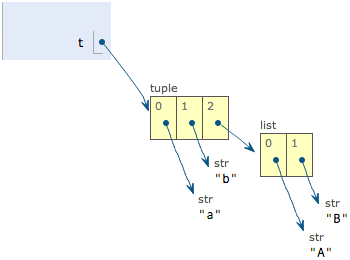
\includegraphics[width=0.6\linewidth]{fig/9239735167876800.png}
\end{figure}


当我们把 list
的元素\texttt{\textquotesingle{}A\textquotesingle{}}和\texttt{\textquotesingle{}B\textquotesingle{}}修改为\texttt{\textquotesingle{}X\textquotesingle{}}和\texttt{\textquotesingle{}Y\textquotesingle{}}后,tuple
变为:

 
 \begin{figure}[htp]
	\centering
	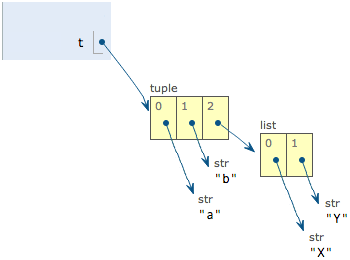
\includegraphics[width=0.6\linewidth]{fig/9239736475158720.png}
\end{figure}


表面上看,tuple 的元素确实变了,但其实变的不是 tuple 的元素,而是 list
的元素。tuple 一开始指向的 list 并没有改成别的 list,所以,tuple 所谓的
``不变'' 是说,tuple
的每个元素,指向永远不变。即指向\texttt{\textquotesingle{}a\textquotesingle{}},就不能改成指向\texttt{\textquotesingle{}b\textquotesingle{}},指向一个
list,就不能改成指向其他对象,但指向的这个 list 本身是可变的!

理解了 ``指向不变'' 后,要创建一个内容也不变的 tuple
怎么做?那就必须保证 tuple 的每一个元素本身也不能变。

\hypertarget{ux7ec3ux4e60}{%
\subsubsection{练习}\label{ux7ec3ux4e60}}

请用索引取出下面 list 的指定元素:

\begin{pythoncode}
# -*- coding: utf-8 -*-

L = [
    ['Apple', 'Google', 'Microsoft'],
    ['Java', 'Python', 'Ruby', 'PHP'],
    ['Adam', 'Bart', 'Lisa']
]
\end{pythoncode}

\hypertarget{ux5c0fux7ed3}{%
\subsubsection{小结}\label{ux5c0fux7ed3}}

list 和 tuple 是 Python
内置的有序集合,一个可变,一个不可变。根据需要来选择使用它们。

\hypertarget{ux53c2ux8003ux6e90ux7801}{%
\subsubsection{参考源码}\label{ux53c2ux8003ux6e90ux7801}}

\href{https://github.com/michaelliao/learn-python3/blob/master/samples/basic/the_list.py}{the\_list.py}

\href{https://github.com/michaelliao/learn-python3/blob/master/samples/basic/the_tuple.py}{the\_tuple.py}

